\documentclass[11pt,a4paper]{report}
\usepackage[utf8]{inputenc}
\usepackage[T1]{fontenc}
\usepackage{lmodern}
\usepackage[french]{babel}
\usepackage{amsmath}
\usepackage{graphicx}
\usepackage{geometry}
\usepackage{pdflscape}
\usepackage{pdfpages}
\geometry{margin=2.5cm, headheight=14pt}
\usepackage{parskip}
\usepackage{setspace}
\usepackage{fancyhdr}
\usepackage{hyperref}
\usepackage{qrcode}

% Configuration des en-têtes et pieds de page
\pagestyle{fancy}
\fancyhf{}
\fancyhead[L]{\small\textit{Souvenirs de jeunesse}}
\fancyhead[R]{\small\textit{Chapitre \thechapter}}
\fancyfoot[C]{\thepage}
\renewcommand{\headrulewidth}{0.4pt}
\renewcommand{\footrulewidth}{0pt}

% Numéro de release injecté par le workflow ; valeur locale par défaut.
\providecommand{\releaseversion}{Version de développement}

\begin{document}

\begin{titlepage}
    \centering
    \vspace*{1.5cm}
    {\Huge \textbf{Souvenirs de jeunesse}\par}
    \vspace{1cm}
    {\Large \textbf{Félix Berloty}\par}
    \vspace{0.6cm}
    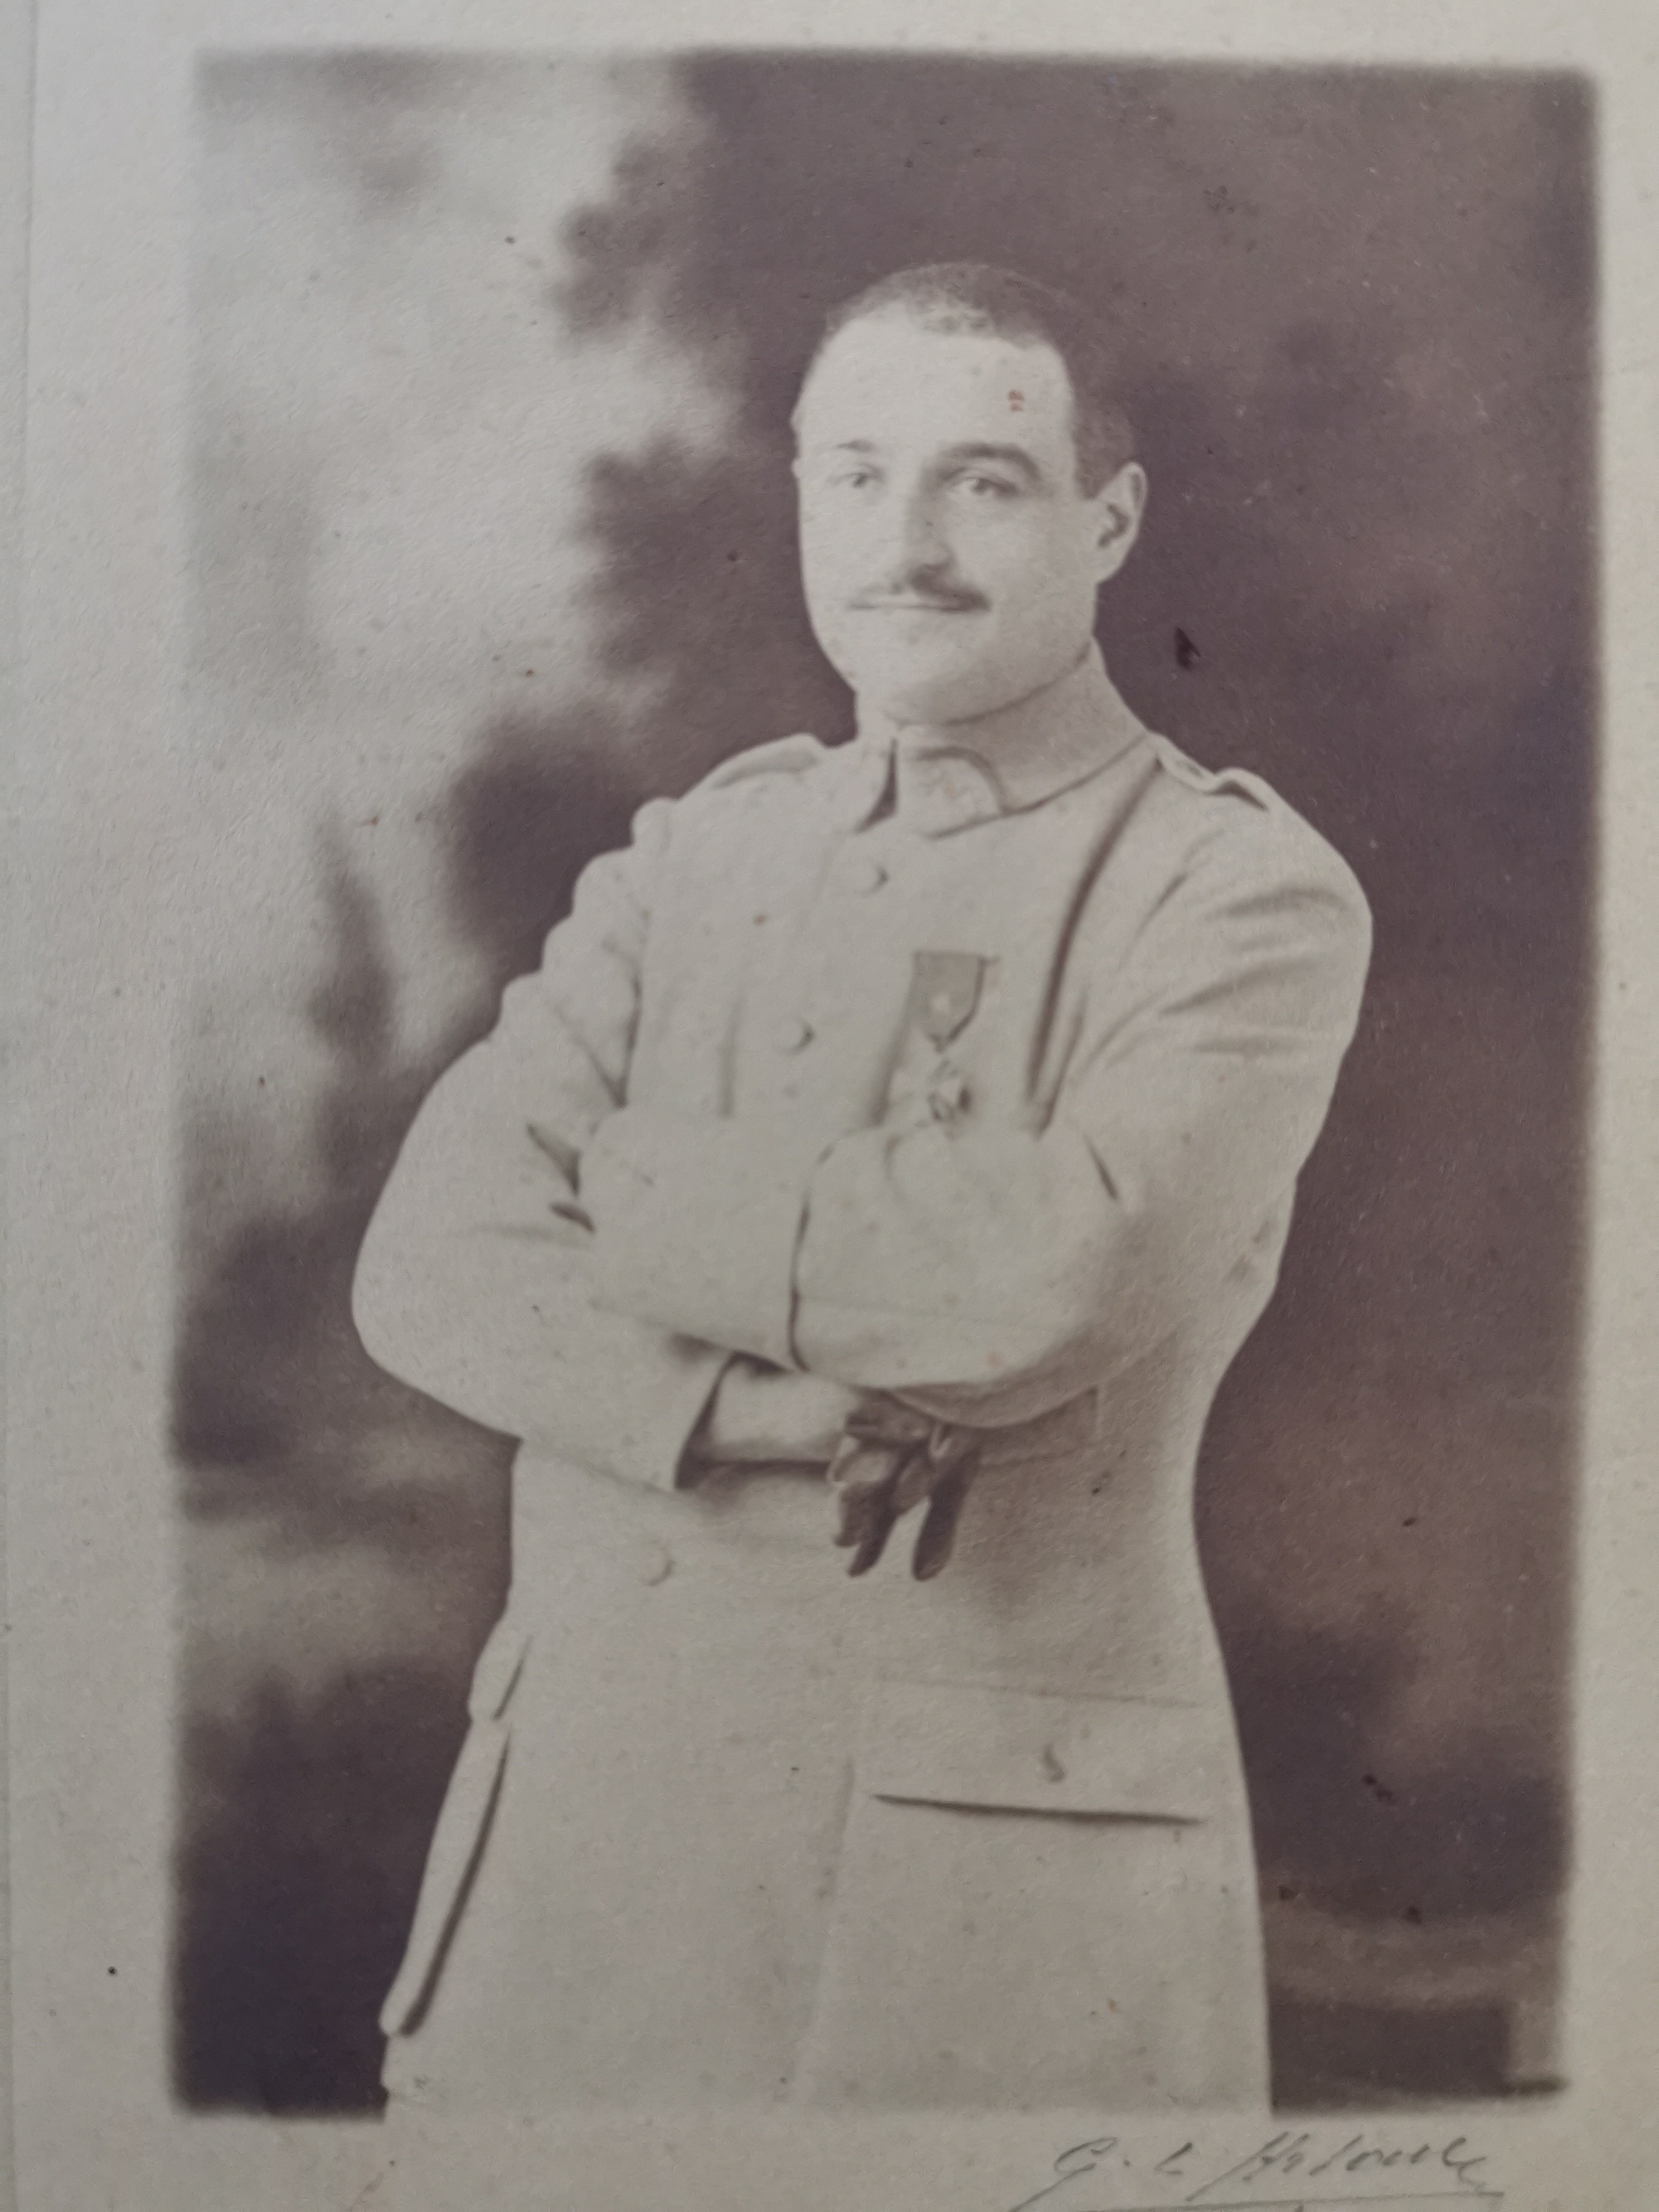
\includegraphics[height=8cm,keepaspectratio]{Illustrations/Portrait_Felix_Berloty.jpg}\par
    \vspace{0.6cm}
    {\small \textit{Félix Berloty (1886--1951)}\par}
    \vfill
    \begin{flushright}
        {\scriptsize \textit{\releaseversion}\par}
    \end{flushright}
\end{titlepage}

\newpage
\pagestyle{plain}
\tableofcontents
\newpage

\chapter*{Note du transcripteur}
\addcontentsline{toc}{chapter}{Note du transcripteur}

La présente transcription a été réalisée à partir du tapuscrit dactylographié de \textit{Souvenirs de jeunesse} de Félix Berloty (1886--1951), conservé dans nos archives familiales. Le document original compte soixante-treize vues numérisées : une page de couverture et soixante-douze pages de texte, couvrant la période 1886--1914 environ.

La transcription a été réalisée à l'aide du modèle Gemini 3.1 Pro (outil \texttt{agy}), en lecture visuelle directe des scans à haute résolution. Les erreurs mécaniques du tapuscrit (lettre \texttt{I} tapée à la place du chiffre \texttt{1}, espacements et césures de la machine à écrire) ainsi que les erreurs de syntaxe et d'orthographe manifestes ont été corrigées. Le vocabulaire, les tournures d'époque et les graphies des noms propres sont conservés. Malgré les vérifications effectuées, des erreurs de transcription peuvent toutefois subsister.

Toute erreur relevée peut être signalée sur la page GitHub du projet :

\begin{center}
    \href{https://github.com/grostim/FelixBerloty/issues}{\textbf{Signaler une erreur de transcription sur GitHub}}

    \vspace{0.5cm}
    \qrcode[height=3cm]{https://github.com/grostim/FelixBerloty/issues}
\end{center}

Les corrections seront intégrées lors d'une prochaine actualisation de la transcription. Le QR code ci-dessus renvoie vers cette même page afin de faciliter le signalement depuis la version imprimée.

Les versions actualisées de ce document, au format PDF et au format EPUB --- adapté aux liseuses et autres lecteurs numériques --- sont disponibles sur le dépôt GitHub du projet :

\begin{center}
    \href{https://github.com/grostim/FelixBerloty/releases/latest}{\textbf{Consulter les versions actualisées sur GitHub}}
\end{center}

\vfill
\begin{flushright}
    {\scriptsize \textit{Document familial --- usage privé}}
\end{flushright}
\newpage

% ===================================================
% CHAPITRE 1 — Page 1
% ===================================================
\chapter{Naissance et Enfance (1886--1890?)}

\section*{Naissance et Enfance}

Je suis né le 15 Août 1886, vers 23 hrs 30, à Lyon 5me arrondissement, Montée des Carmes Déchaussés, au-dessus de la gare St Paul.

Mes parents, qui avaient une grande dévotion à la Ste Vierge, se réjouirent de cette coïncidence de ma naissance avec la grande fête mariale et y voyaient volontiers, comme une marque de sa protection à mon égard.

Ma naissance fut, m'a-t-on toujours dit, bien accueillie. J'étais, en effet le premier garçon, héritier du nom, dans le ménage de mes parents, mariés depuis 11 ans et j'étais séparé de ma soeur Marie par un intervalle de 8 ans.

On m'a souvent raconté que, mon arrière grand'mère paternelle, née Bonaventure POULAT et morte trois ans plutôt à 97 ans, dans un état excellent de conservation jusqu'à 95 ans, exprimait souvent ses regrets de l'absence d'héritier mâle ; elle en était même si peinée qu'elle appelait ma soeur Marie ``le Petit''.

Je fus déclaré à la mairie du 5me, le lendemain de ma naissance, par mon père assisté de mon grand père Romain DEMOUSTIER, ancien agent de change à Lyon et de mon cousin Paul MADINIER, mari de ma cousine BOFFARD, alors clerc à l'étude ; ceci ne l'a pas empêché de faire plus tard sa médecine et de prendre son titre de docteur. Il exerça cette profession assez longtemps (vers 1900--1920) dans le quartier de St Just et du Point du Jour.

Je fus baptisé quelques jours plus tard, dans l'église paroissiale de St Paul. Je reçus au baptême les prénoms de Joseph, Jean, Marie Felix ; les deux prénoms de Joseph et Marie par dévotion, celui de Jean en raison de mon parrain, Jean dit Joanny BOFFARD, mon oncle par suite de son alliance avec ma tante Joséphine BERLOTY, sa soeur aînée de 10 ans de mon père.

Mon oncle BOFFARD était aussi le prédécesseur de mon père comme notaire à Lyon. Très bon, très empressé à rendre service, il en avait rendu d'importants à la mort de mon grand père et s'était acquis, à ce titre, une position particulière dans la famille. Enfin le nom de Felix, que je devais porter dans l'usage courant, me fut donné en souvenir de mon grand père paternel, qui fut le premier notaire du nom, à Lyon de 1840 à 1871 et qui par son activité, son travail et son esprit d'entreprise, fut le véritable fondateur de notre famille.

% NOTE SÉQUENCAGE : la numérotation des scans suit l'ordre du carnet à spirale,
% pas l'ordre de lecture : la page 02 précède matériellement la page 03, mais le
% texte s'enchaîne de 03 vers 02 (les raccords sont vérifiés). Ordre logique : 1, 3, 2, 4, 5...

% --- Page 3
Ma marraine fut ma grand'mère DEMOUSTIER que, personnellement, je n'ai jamais connue, car elle mourut quelques jours après ma naissance d'une crise cardiaque.

% --- Page 3
A cette époque, mes parents partageaient leur vie, entre trois résidences habituelles, comme, d'ailleurs, un certain nombre de personnes de leurs relations.

% --- Page 3
1ère) Place de la Bourse 2, où ils occupaient de Novembre à Mai, un appartement de 7 à 8 pièces au 2me étage, au-dessus de l'étude ; l'autre côté de l'étage, composé de 4 à 5 pièces était réservé à mes grands-parents DEMOUSTIER et relié à notre appartement dont il était distinct cependant.

% --- Page 3
2me) Montée des Carmes déchaussés. C'est là où je suis né, dans une maison que mes parents tenaient en location des Pères maristes. C'était une demi-campagne, où ils passaient la mi-saison au printemps et à l'automne.

% --- Page 3
3me) Enfin Gros Bois où ma Mère et plus tard nous-mêmes nous rendions pour les grandes vacances et quelquefois à Pâques.

% --- Page 3
Chacune de ces maisons était meublée, les déménagements consistaient simplement dans le transport d'une malle et d'un peu de linge.

% --- Page 3
Mes grands-parents DEMOUSTIER habitaient pendant l'hiver à Lyon, en face de notre appartement. Si mes souvenirs sont exacts, ils y avaient succédé à mon arrière-grand'mère BERLOTY morte en 1883.

% --- Page 3
Je rappelle que cette maison appartenait à ma tante BOFFARD, qui l'avait acquise de la succession de son père ; lui-même, l'avait fait construire vers 1850, à l'époque des constructions de la rue Impériale dont il fut, avec Mr. de BOISSIEU et d'autres l'un des fondateurs ; on racontait même, dans le public, qu'elle représentait les honoraires qui lui étaient dus pour ses démarches et les actes qu'il reçût pour la Société dont il était le notaire.

% --- Page 3
L'été mes grands-parents DEMOUSTIER allaient s'installer dans la propriété qu'ils possédaient à Lyon, 62 chemin de la Favorite, à l'angle du chemin de la Favorite et du chemin de l'Etoile d'Alaÿ.

% --- Page 3
Cette propriété qui est devenue, aujourd'hui, celle du Syndicat des Institutrices privées, était moins grande à l'époque, mais devait déjà avoir 4 ou 5 hectares.

% --- Page 3
La maison de construction assez légère, était cependant, assez confortable pour le moment. Elle comportait un grand vestibule d'entrée, à gauche un petit salon, à droite une salle à manger, derrière cuisine et office, et au fond donnant sur la façade nord, il y avait un grand salon dont on profitait rarement.

% --- Page 3
Il y avait également dans le jardin des dépendances, écurie, remise, orangerie, trois serres, maison du jardinier et une autre petite maison de maître, avec un billard où mon oncle et ma tante Elysée DEMOUSTIER-BILLET (frère de ma mère) s'installaient parfois en ménage. Au 1er étage de la maison principale se trouvait un certain nombre de chambres dont celle de mon grand'père et une chapelle, assez bien meublée et décorée. Le long du chemin de l'Etoile d'Alaÿ, presqu'à la naissance du chemin de la Favorite se trouvait une petite maison de 2 pièces, fort bien installée, où ma Mère jeune, s'amusait à faire la cuisine ; tradition qu'avec les enfants DEMOUSTIER nous conservâmes alors que nous étions jeunes.

% --- Page 03 (fin) + Page 02 (début) — phrase continue
Si j'ai rappelé ces souvenirs avec un certain détail, c'est en raison du rôle qu'a joué, pour nous, cette propriété où nous nous rendions toujours avec un grand plaisir, et où s'est écoulé une grande partie de ma jeunesse, quoique je n'y ai jamais séjourné autrement qu'en passant.

% --- Page 2
Le parc, très bien entretenu par mon grand'père qui s'y intéressait beaucoup, et par 2 jardiniers, comportait, dans les parties supérieures et inférieures, deux parcelles cultivées en jardin potager et fruitier. Mon grand'père aimait beaucoup la culture des fruits ; c'était l'époque de la méthode GRESSENT, que mon grand père avait spécialement étudiée et qu'il prisait beaucoup.

% --- Page 2
Je me rappelle qu'il y avait toujours sur la table et dans ses appartements, de très belles fleurs, ou plantes et de très beaux et bons fruits, en particulier, des poires, raisins, fraises, framboises.

% --- Page 2
Le milieu de la propriété était planté d'après un dessin, disait-on, de Le Notre, de très beaux marronniers et orné par un grand bassin et des statues diverses. Il y avait notamment un rond point dit des quatre saisons, auquel aboutissaient de grandes allées couvertes de petits cailloux ronds et bordées de très beaux et grands arbres. Le défaut de cette propriété était le manque de vue à peu près complet ; une seule petite échappée qui malheureusement laissait apercevoir le cimetière de Loyasse.

% --- Page 2
Dans la partie basse de la propriété, le long du chemin de la Favorite, en face d'un portail à claire voie, il y avait un petit parc grillagé où on élevait des daims et des biches. En dessous, se trouvait une magnifique volière où ma Mère me racontait avoir vu de superbes oiseaux d'eau, mandarins, carolins, cygnes, cigognes, etc., mais pour ma part, je n'y ai connu que de petits oiseaux : canaris, cardinaux, perruches et peut-être quelques faisans.

% --- Page 2
Au Nord Est de la propriété, dans le bas, il y avait un quadrilatère de terrain d'un hectare environ, qui reliait en quelque sorte la partie centrale de la propriété au chemin des Grandes Terres qui longeait cette partie. On y faisait de la culture de potager et de verger. Un portail permettait de sortir par là de la propriété à pied et en voiture. Cette sortie était utilisée fréquemment, par les personnes qui se rendaient à Vaise ou dans la propriété de Champvert, appartenant aux BRUNET-LECOMTE.

% --- Page 2
Ma mère m'a raconté souvent, dans mon enfance, que c'est en revenant de chez ma tante que ma grand'mère DEMOUSTIER, à la suite d'une frayeur causée par un âne attelé à une petite voiture, au moment où elle franchissait le portail, prit une fatigue cardiaque qui l'emmena, je crois, le soir même. C'était peu de temps après ma naissance et ce fut l'occasion de la première sortie de ma mère.

% --- Page 2
C'était le 25 Septembre 1886.

% --- Page 2
Mes grands parents DEMOUSTIER avaient eu de leur union, cinq enfants dont quatre vivaient alors :

% --- Page 02 (fin) — liste des cinq enfants
1) Elysée, marié à Melle Marguerite BILLET, qui avait lui-même à l'époque 4 fils \\ \hspace*{2em} Romain, décédé vers 1892 \\ \hspace*{2em} Joseph \\ \hspace*{2em} Emmanuel, qui devint jésuite et mourut sur le champ de bataille vers Arras en 1914. \\ \hspace*{2em} Adrien, qui devint lui aussi, plus tard, agent de change à Lyon, successeur de son père et de notre grand'père. Je n'avais que 2 ans et demi d'écart avec lui ;

% --- Page 04 (début) — suite de la liste
2) Une fille Christine, décédée en 1882, première épouse de mon oncle Joseph BRUNET-LECOMTE, qui fut fabricant de soieries et juge au Tribunal de Commerce. Elle laissait deux enfants \\ \hspace*{2em} René, mort capitaine d'infanterie, en 1914, au sud de Verdun \\ \hspace*{2em} b) Marguerite Marie, morte à 20 ans de la fièvre typhoïde.

% --- Page 4
3) Ma Mère

% --- Page 4
4) Hélène, religieuse du Cénacle.

% --- Page 4
5) Elisabeth, qui s'était mariée peu de temps avant avec son beau-frère Joseph Brunet-Lecomte.

% --- Page 4
Du côté de mon Grand Père DEMOUSTIER, je n'ai jamais connu de parents rapprochés, autres que ceux cités ci-dessus.

% --- Page 4
Par contre, ma Grand'mère, née Marie PHELIP, et qui venait de mourir, laissait un frère, mon oncle PHELIP, père de deux fils : Elysée et Gabriel ; et trois soeurs Mmes DUBOST, RICHARD et TREPPOZ.

% --- Page 4
C'est au milieu de ces différents parents qu'allait s'écouler ma jeunesse.

% --- Page 4
Des années de ma tendre enfance, je n'ai pas grand chose à rapporter. Je grandis entouré de la sollicitude de mes parents, dans les résidences rappelées ci-dessus.

% --- Page 4
La propriété, où j'avais vu le jour, avait été abandonnée par mon Père, peu de temps après ma naissance et remplacée par une autre près de Fourvière, rue du Juge de Paix. Cette dernière appartenait au Calvaire des Hommes, dont elle était contiguë ; de l'autre côté, elle était limitée par la propriété de MONICAULT (actuellement des Pères Franciscains et de Paul TREPPOZ) et enfin par la rue du Juge de Paix, sur laquelle donnait une petite terrasse d'où, par temps clair, nous avions une fort belle vue sur la partie sud de Lyon et au-delà, les Alpes du Dauphiné. Toujours en bordure de la rue du Juge de Paix, en face de la propriété des Soeurs de St Joseph, se trouvait la maison d'habitation, dont la vue était malheureusement obstruée des deux côtés.

% --- Page 4
Il serait difficile de se rendre compte de ce que fut ma jeunesse par une comparaison avec la vie de mes enfants aujourd'hui. Sans doute, nous trouverions des points de contact, mais à côté, que de différences dues aux progrès scientifiques, à l'amélioration du confort et des moyens de communication (progrès que j'essaierai de résumer dans un chapitre plus loin), mais, hélas, dues aussi à la cherté actuelle de la vie et aux difficultés que nos maîtresses de maison connaissent, aujourd'hui, mieux que personne.

% --- Page 4
La vie était alors facile et bon marché. Il suffisait à la ménagère de se rendre sur le marché ou dans les magasins pour y trouver, à des prix bien établis et raisonnables tout ce qui lui était utile. Sans doute, les gains étaient limités et modestes, mais la dépense l'était aussi, et surtout cette superposition d'impôts, qui pour être quelquefois occulte, n'en existe pas moins partout, ne rendait pas alors la vie si difficile dans toutes les classes sociales ; de même la liberté commerciale était pratiquée dans tous les domaines.

% --- Page 4
Mes parents avaient, à ce moment-là, à leur service quatre domestiques.

% --- Page 5
Une cuisinière, une femme de chambre, une bonne d'enfants et un valet de chambre. Ce dernier couchait à l'étude, et nettoyait celle-ci entre 6 hrs du soir et 8 hrs du matin. Ce dernier travail n'était pas une sinécure ; il n'était pas question à l'époque d'éclairage électrique, tous devaient s'éclairer au moyen de lampes à huile. C'étaient donc 15 à 20 lampes à huile dont il fallait nettoyer les verres chaque soir, qu'il fallait mécher et garnir -- les lampes à pétrole étaient considérées comme dangereuses et n'étaient pas employées --

% --- Page 5
C'est un de mes vieux souvenirs que cette rangée de lampes qu'on remplissait régulièrement, dans un petit local à la porte des W.C.

% --- Page 5
Il y avait également le chauffage à entretenir. Nous avions quelques poêles à l'étude ou dans l'appartement, mais, en outre, il existait, dans la cave, un chauffage à eau chaude commun aux deux étages. Il n'y avait pas de radiateurs, comme actuellement, mais simplement de gros tuyaux remplis d'eau chaude qui couraient dans des caniveaux recouverts de grilles tout autour des pièces et des vestibules. Il existait en général dans les pièces des cheminées qu'on utilisait par grands froids. Grâce à ce chauffage, qu'on n'utilise plus aujourd'hui sous cette forme, une température très agréable régnait à l'étude et dans notre appartement.

% --- Page 5
Mon Père était très occupé par ses occupations professionnelles.

% --- Page 5
Il descendait généralement à son étude le matin à 8hrs, après avoir assisté à la messe à St Bonaventure à 6hrs 1/2 ou 7 hrs ; il remontait déjeuner à midi et reprenait l'étude à 1 hrs 1/2 jusqu'à 6hrs. Nous dînions à 7hrs du soir. Dans quelques autres familles, notamment chez les Rambaud, on dînait même à 6hrs 1/2.

% --- Page 5
Après dîner, quand nous eûmes un peu grandi, nous restions quelques moments avec nos parents, puis vers 9hrs du soir, on nous faisait coucher. Eux-mêmes en général ne veillaient pas tard.

% --- Page 5
Mon Père recevait volontiers quelques amis ou clients qui venaient le voir à l'étude et qu'il retenait à déjeuner. Certains étaient presque des habitués. Parmi eux deux ecclésiastiques venaient fréquemment.

% --- Page 5
I) Notre cousin Monseigneur Stanislas NEYRAT, protonotaire apostolique, doyen du chapitre de Lyon, titre dont il était très fier. Il entretenait les meilleures relations avec mon père, en raison de notre parenté d'abord, mais surtout en raison de leurs rapports qui remontaient assez loin en arrière, au temps où il avait conduit mon père et quelques autres jeunes gens de son âge, en Espagne et au Portugal. Ils avaient fait ce voyage en grande partie à pied, traversant le pays du Nord au Sud.

% --- Page 5
Au cours de ce voyage, dont le souvenir revenait souvent dans la conversation, l'abbé NEYRAT était tombé gravement malade ; ses autres compagnons l'avaient abandonné en raison de leurs obligations qui les rappelaient en France, mon père seul, encore jeune, était resté auprès de lui et l'avait soigné avec beaucoup de dévouement. L'Abbé NEYRAT lui en était resté profondément reconnaissant.

% --- Page 6
C'était un homme de 20 à 25 ans plus âgé que mon Père, fort distingué, excellent musicien ; il avait été maître de chapelle de St Jean et à son heure devenait organiste et même compositeur. Au demeurant, il était aimable, lisait beaucoup et était voyageur dans l'âme. Marcheur infatigable, il faisait facilement sans repos 80 et même 100 Kms. Il me racontait qu'il venait à pied de Feurs dans la Loire et qu'un trajet de cette importance ne comptait pas pour lui, au point qu'en arrivant à Lyon, il faisait encore plusieurs visites. Il disait connaître toutes les capitales d'Europe, à l'exception, je crois, d'une.

% --- Page 6
Plus tard, aimant moi-même beaucoup les voyages, je l'interrogeais avant de me mettre en route, il répondait très volontiers et nous donnait toujours des renseignements intéressants et précieux ;

% --- Page 6
C'était un esprit fin et distingué, en apparence très doux, mais dans le fond énergique et sachant bien ce qu'il voulait. À la suite des voyages qu'il organisait avec des jeunes gens, comme ceux qu'il fit avec mon Père en Espagne, avec mon oncle Élysée Demoustier et mon oncle Bonaventure BERLOTY (depuis Jésuite) en Russie, ses anciens compagnons le désignaient souvent sous le nom de ``Capitaine'' ; ce qui rappelle bien son caractère de chef dans ses déplacements.

% --- Page 6
L'abbé NEYRET a appartenu à l'Académie de Lyon ; il a écrit un certain nombre de récits de voyages : voyage en Espagne, voyage au Mont Athos que nous avons à Gros Bois etc et quelques recueils de cantiques religieux dont il avait composé la musique.

% --- Page 6
L'autre ecclésiastique qui venait fréquemment, était l'Abbé (depuis chanoine) BOISARD. Ce dernier était vaguement parent de mon oncle BOFFARD. Il avait débuté dans la vie en faisant ses études de pharmacien, puis entré dans les ordres, il s'était intéressé aux questions sociales et principalement à la formation de la jeunesse ouvrière. C'est ainsi qu'il avait créé en 1882 les Ateliers d'apprentissage qui fonctionnaient à Lyon cours Gambetta, sous sa direction et celle de quelques prêtres de ses amis. Il y recevait des jeunes gens de condition modeste, en pension et les formait à la menuiserie, à la serrurerie, et au métier de cordonnier. Plus tard, l'affaire prit de l'extension, et mon Père s'est adressé, plusieurs fois, à lui pour différents travaux, notamment pour les bancs de l'Église d'Ouroux et notre bibliothèque de Gros Bois.

% --- Page 6
À l'époque de mon enfance, il avait aussi dans le même but ouvert une école d'apprentissage agricole et de colonisation à Ste Marie du Zit (Tunisie) où il allait régulièrement passer quelques semaines chaque année.

% --- Page 6
C'était un sujet de conversation qui revenait souvent avec mon Père, qui s'intéressait à son oeuvre et avait avec lui des rapports.

% --- Page 6
Ces visites qui étaient loin d'être moroses, égayaient et variaient nos repas. Notre ordinaire même en profitait plutôt, car elles nous valaient souvent quelques plats ou quelques boissons supplémentaires. C'est ainsi que le souvenir de l'Abbé NEYRET est lié quelque peu à celui des huîtres que mon Père achetait pour lui, le matin à la criée aux halles et au petit vin blanc qui les accompagnait normalement.

% --- Page 7
Je l'ai dit, la vie était facile à cette époque.

% --- Page 7
Sans faire un luxe extraordinaire, nous avions un ordinaire soigné et abondant. C'est ainsi, que nous avions normalement, à chaque repas de midi et du soir, deux plats de viande, ou une entrée d'oeufs et un poisson, (soles, saumon, langouste, homard) et un plat de légumes, généralement : pommes de terre, petits pois, haricots verts, épinards, et des fruits. Nous avions aussi souvent des entremets.

% --- Page 7
Pour l'approvisionnement nous étions très bien placés, à deux pas des halles centrales et du marché du quai St Antoine ou du grand charcutier de l'époque Watebled, qui était rue de la Bourse ; en face de la place du même nom, et au-dessus du restaurant Moderne où mon Père faisait souvent prendre de la bière en broc.

% --- Page 7
Tout cela, je l'ai dit, à des prix abordables. Pour en donner une idée, je dirais qu'un bon repas, à l'époque, dans un très bon restaurant, pouvait coûter normalement, de 2 à 5 francs.

% --- Page 7
Vers 1890, je fus atteint d'une bronchite qui rétrocédait lentement.

% --- Page 7
Sur les conseils de notre médecin, le vieux docteur Marduel, qui tout en étant assez simple de manières, venait à la maison, en redingote, en gibus, avec un gros lorgnon en écaille, mes parents décidèrent de m'emmener passer quelque temps à Montreux. C'est ainsi, que pour la première fois, je franchis la frontière Suisse que je devais, dans la suite, franchir si souvent. (J'avais 4 ans)

% --- Page 7
J'ai gardé, pour mon âge, un souvenir très présent de ce premier séjour hors de chez moi, et je revois même actuellement, l'hôtel et la chambre où j'étais installé avec mes parents, au-dessus du lac de Genève. Les petits déjeuners du matin étaient déjà à cette époque, très appréciables. Cela constitue certainement un de mes plus anciens souvenirs.

% --- Page 7
Nous rentrions donc à Lyon, enchanté pour ma part, de ce déplacement que j'ai toujours eu plaisir à renouveler.

% --- Page 7
Le 13 Septembre 1890, se place la naissance de ma soeur Elisabeth à Lyon 2me.

% --- Page 7
Mon Père étant très pris par ses affaires, c'est surtout ma Mère, comme cela arrive souvent, qui s'est occupée de moi pendant mon enfance.

% --- Page 7
Aidée quelquefois par l'institutrice de ma soeur Marie, Mademoiselle VERRIER, elle m'apprit à lire et à écrire et quelques éléments d'instruction religieuse.

% --- Page 08 (fin) + Page 09 (début) — phrase continue
Ces souvenirs de la guerre de 1870 étaient encore bien récents au moment de ma jeunesse, et présents dans tous les esprits ; c'est dire que son évocation me revient souvent quand ma pensée se reporte à cette époque.

% --- Page 9
Tous ceux qui avaient assisté à notre défaite, en avaient été consternés, et je puis dire que jusqu'en 1914, cette pensée était constamment présente à l'esprit de tous ceux qui s'intéressaient à l'avenir de la France. Si l'esprit de revanche n'existait pas, du moins tous étaient hantés par la volonté de pouvoir, le cas échéant, opposer à l'envahisseur une armée forte, si l'occasion se présentait à nouveau. Cette formation de nos chefs et de la jeunesse à laquelle j'ai appartenu, ne fut certainement pas étrangère à nos succès de 1914--1918.

% --- Page 9
Mon Père n'avait un peu de temps libre à nous consacrer que le Dimanche, car il n'était pas question alors de semaine anglaise et d'après-midi du Samedi libre.

% --- Page 9
Je ne me privais pas non plus, de l'interroger, cependant, sur sa famille et sur son jeune temps. Il parlait volontiers de son père, de son activité dans le notariat à une période, celle du second Empire, qui a correspondu pour la France à un grand développement et à une prospérité nouvelle du fait des applications de la vapeur à l'Industrie et à la Locomotion. Il ne faut pas perdre de vue que les chemins de fer s'étaient beaucoup développés de 1840 à 1870, laps de temps pendant lequel mon grand-père fut notaire à Lyon.

% --- Page 9
Ce dernier, très entreprenant, très actif, presque trop audacieux, s'était créé une très belle clientèle, peut-être un peu grâce à sa femme, née Coste, qui était apparentée aux Colomb de Gaste et par là à tout un milieu riche et commerçant de Lyon et de la région.

% --- Page 9
Mais son champ d'action s'étendait beaucoup plus loin ; c'est ainsi qu'il ne se contenta pas à Lyon de promouvoir la création de la Rue Impériale, mais qu'il alla chercher fortune, sans des résultats bien certains, dans la construction de la ville de Rouen et même dans celle du Port de Cadix (Espagne) !

% --- Page 9
Cette dernière oeuvre s'explique par la prospérité, à l'époque, de certaines affaires Espagnoles. Beaucoup de Lyonnais s'étaient intéressés alors aux chemins de fer de ce pays. C'est ainsi que pendant longtemps, à Lyon, nous rencontrions souvent dans les portefeuilles de nos concitoyens, jusqu'en 1914, des titres des Sociétés de Nord-Espagne, d'Ouest-Espagne, Madrid Cacéres, Barcelone directe etc. On s'explique donc, assez facilement que mon grand-père, en homme entreprenant qu'il était, ait pu miser sur le développement de ce port qui était le point le plus au Sud-Est de l'Europe en direction de l'Amérique latine.

% --- Page 10
Malheureusement, il n'avait pas compté sur le tempérament Espagnol et cette entreprise se termina assez mal.

% --- Page 10
Heureusement, mon grand-père avait d'autres cordes à son arc. C'était un terrien dans l'âme, et non seulement il avait à Lyon une ou deux maisons dont la place de la Bourse, mais il était devenu propriétaire de nombreuses propriétés rurales.

% --- Page 10
J'en cite quelques-unes : Gros Bois (non seulement notre part, mais celle des BOFFARD, actuellement MOLLARD, et celle des RAMBAUD - environ 600 hts-) Lantigné-Vougy-Montcarrat, acheté depuis par les Thomasset, près de Bourgoin- Pressy sous Dun-Claveisolles (propriété actuelle des RAYMOND)

% --- Page 10
Mon Père m'entretenait souvent aussi de la guerre de 1870.

% --- Page 10
Lui-même était trop jeune pour être mobilisé ; cependant la guerre se prolongeant, il hésitait à partir lui-même en s'engageant, mais avant de signer son engagement, il voulut aller embrasser sa grand'mère qui était partie elle aussi à Fribourg.

% --- Page 10
Avant son retour, l'armistice était signé, si bien que sa classe ne fut jamais appelée et qu'à part quelques périodes de réserviste qu'il fit plus tard, il ne porta jamais l'uniforme.

% --- Page 10
Mon grand'père BERLOTY mourut en 1871, entouré de l'affection et les soins que lui donnait mon Père ; il avait malheureusement pris une crise d'urémie et de la furonculose, maladie qui, à l'époque, laissait peu d'espoir.

% --- Page 10
Avant sa mort, il avait marié sa fille aînée Joséphine, à celui qui fut depuis mon oncle BOFFARD et qui, devenu le successeur de mon grand-père comme notaire à Lyon, fut mobilisé quelques temps, mais qui, je crois, ne quitta pas Lyon. Il m'a raconté qu'il fut affecté à la Garde Nationale et que son principal service consistait à prendre la faction devant la Banque de France, à deux pas de son étude.

% --- Page 10
J'ai rappelé le voeu des Lyonnais, d'édifier une nouvelle et grande église à la Ste Vierge, sur la colline de Fourvières, près de l'ancienne devenue trop petite, si la ville de Lyon était épargnée pendant la guerre. Celle-ci terminée, une commission se constitua vite pour réaliser ce voeu. Aussi quand nous nous établîmes pour l'été à Fourvières, rue du Juge de Paix, les travaux étaient depuis longtemps commencés. Cependant je me rappelle très bien la nouvelle église, non encore consacrée et dont le gros oeuvre était encore en cours d'achèvement.

% --- Page 11
Nous habitions à deux pas, et souvent, surtout pendant le mois de Mai, nous nous rendions le soir, avec ma Mère, à l'ancienne église, seule ouverte alors, pour assister au Salut ou à une cérémonie religieuse. Cette église était alors plus grande qu'elle n'est actuellement. Non seulement la nef actuelle était plus longue, car la chapelle actuelle de St Thomas, qui est derrière l'autel en faisait partie, mais elle était doublée par une autre nef semblable sur laquelle on a pris depuis l'escalier et la sacristie de la nouvelle église. Cette deuxième nef était alors consacrée à St Thomas qui se trouve maintenant relégué dans la chapelle derrière.

% --- Page 11
Plus tard fut consacrée la grande église, je me rappelle très bien y avoir assisté du haut des tribunes. Ce fut une très belle cérémonie, présidée par le Cardinal COUILLÉ et le Cardinal RICHARD archevêque de Paris assisté de nombreux archevêques, évêques ou abbés mitrés. Je me rappelle aussi avoir assisté une autre fois à une grande cérémonie, dans la nouvelle basilique, à l'occasion du baptême des cloches, gros bourdon et carillon. Toutes étaient rangées en lignes, le long du couloir central. Mon grand père Demoustier et ma Mère étaient parrain et marraine d'une de ces cloches et sauf erreur leurs noms doivent être gravés dans le bronze de cette cloche.

% --- Page 11
Nous nous rendions aussi assez souvent avec ma Mère assister aux offices chez les Dames du Cénacle, place de Fourvières où était religieuse une de mes tantes : Hélène DEMOUSTIER. Cette dernière était un peu plus jeune que ma Mère. C'était une petite personne un peu boulotte, qui riait constamment ; au demeurant la meilleure personne du monde, très empressée quand nous allions lui rendre visite ; ce qui ne signifie pas qu'elle fût très débrouillarde.

% --- Page 11
Été comme hiver, nous allions dîner tous les jeudis soirs chez mon Grand Père DEMOUSTIER, qui nous recevait tous : Demoustier, Berloty, Brunet-Lecomte. C'était pour nous l'occasion de faire un excellent dîner, car mon Grand Père faisait venir une très bonne cuisinière et tenait beaucoup à ce que nous soyons bien et abondamment traités. J'aimais beaucoup ces réunions de famille, qui m'offraient l'occasion d'un bon dîner et d'une agréable soirée en compagnie de mes cousins et cousines Demoustier et Brunet-Lecomte. La réunion était souvent très gaie, ce qui ne l'empêchait pas de se terminer de bonne heure, car à l'époque on se couchait très tôt vers 9 heures et demie. À Lyon, nous n'avions qu'à ouvrir la porte, pour nous retrouver dans le salon de mes parents. À la Favorite, (les autos n'existant pas à cette époque) une voiture de louage, généralement un coupé, venait

% --- Page 12
nous prendre et nous ramener à la maison.

% --- Page 12
Nous aimions beaucoup ces réunions de famille. Les mauvaises langues prétendaient qu'elles ne me réussissaient pas toujours très bien et que par une fâcheuse coïncidence, j'étais souvent malade le vendredi matin, mais la calomnie est si facile.

% --- Page 12
J'aurais voulu, tirant enseignement du plaisir que j'éprouvais à me trouver ainsi avec des cousins et cousines de mon âge, obtenir de mes oncles Rambaud et Boffard, qu'avec mes parents, ils organisent des réunions analogues le Dimanche où nous aurions rencontré le côté de ma famille paternelle. Ce souhait trouva un commencement de réalisations dans les dîners qui nous réunissaient le Dimanche soir, alternativement chez les uns et chez les autres, mais ce succès fut moins affirmé et conserva toujours un caractère précaire. Je me rencontrais cependant fréquemment avec les Boffard, beaucoup plus âgés que moi et surtout avec les Rambaud où André, Emmanuel et Adrien, quoique mes aînés, prenaient part volontiers à mes distractions. (3 Mai 1893, naissance de mon frère Joseph).

% --- Page 12
En 1894, je fus par hasard, témoin de l'assassinat du Président CARNOT. Celui-ci venait à Lyon où de grandes fêtes furent organisées en sa faveur. Il devait notamment dîner, en nombreuse compagnie, à la Chambre de Commerce dans la grande salle du Palais du Commerce où se tient habituellement la Bourse. Mon père était lui-même invité à ce grand banquet en raison de ses fonctions de maire d'Ouroux. Nous étions alors installés à Fourvière, rue du Juge de Paix, mais j'étais jeune et naturellement j'étais intéressé et attiré par ces fêtes ; c'est pour cela que j'avais demandé à mes parents de redescendre à Lyon pour, au moins, assister au défilé rue de la République, des fenêtres de notre appartement. Il en fut ainsi décidé, une première fois tout se passa sans incident. Le soir, le Président devait présider le dîner à la Bourse, puis vers neuf heures du soir se rendre au Grand Théâtre pour assister à une représentation de gala et enfin revenir à la Préfecture, qui avait été récemment inaugurée et où il était installé. Il fut convenu qu'avec ma Mère nous reviendrions assister au défilé à 9 hrs. Vers cette heure-là nous remontions donc à l'appartement et nous nous installâmes à la fenêtre. Mon Père sortant du dîner, qui s'était bien passé, nous y rejoint bientôt. Et quelques instants après nous aperçûmes, remontant la rue de la République, entre deux haies de troupes et de spectateurs, les chevaux de tête de la voiture présidentielle. Ceux-ci s'arrêtèrent et devant eux, un homme traversa la rue pour atteindre la haie de spectateurs qui étaient devant le grand hôtel en passant juste devant la voiture du Président. Il allait se perdre dans la foule, quand il fut rejoint par des inspecteurs en civil qui l'arrêtèrent. Nous n'apercevions pas encore, à ce moment, l'intérieur du landau présidentiel et n'avions pas vu ce qui venait de se passer. Mon Père eut cependant, tout de suite, le sentiment d'un attentat et nous le dit. Quelques instants après, la voiture reprenait sa marche en avant, mais au lieu de continuer sur le Grand Théâtre la police faisait ouvrir la haie de spectateurs qui étaient rangés sur la place de la Bourse et le cortège venait s'arrêter exactement sous nos fenêtres.

% --- Page 13
Le Président, inerte, était couché sur la banquette et autour de lui s'empressaient le Préfet et le Maire. Ce dernier était alors le Docteur Gailleton. Mon Père eut alors la pensée d'offrir son appartement pour abriter le Président. Il nous quitta en disant qu'il allait faire cette proposition, mais quelques secondes plus tard, il remontait en nous disant qu'il n'avait pu approcher de la voiture.

% --- Page 13
Nous avions vu d'ailleurs que celle-ci était isolée alors de toutes sortes de badauds par les gardes républicains et la police. C'est alors que mon père dit à ma mère qu'il se rendait à l'Archevêché prévenir le Cardinal Coullié, qui devait y être rentré, venant lui-même du banquet auquel il avait assisté. De notre côté, nous devions regagner nous-mêmes la rue du Juge de Paix. Ainsi fut fait. Mon Père arrivait à l'archevêché, mais les portes de la grille de la cour par où on y entrait, qui était la cour actuelle de la Bibliothèque, étaient fermées ; mon Père dut donc se rendre chez son ami Monseigneur Déchelette, alors vicaire général qui habitait au N°5 de l'avenue de l'Archevêché d'alors (aujourd'hui avenue Adolphe Max). Le temps de réveiller Monseigneur Déchelette permit à une autre personne qui avait eu la même idée, d'arriver, et plus heureux que mon Père de pénétrer à l'intérieur de l'archevêché et de prévenir le Cardinal, qui se rendit effectivement à la préfecture, où il releva un malheureux petit vicaire de paroisse et administra le Président.

% --- Page 13
Mon Père lui-même se rendait à la Préfecture, mais ne pouvant y rendre aucun service, il nous rejoignait à Fourvières. La nuit fut assez agitée. La foule qui était jusque là très enthousiaste, avait appris que le Président avait été assassiné par un Italien du nom de Caserio. Il s'en suivit un mouvement de phobie contre tous les Italiens établis à Lyon qui furent plus ou moins boycottés. C'est ainsi qu'il y eut pas mal de casse dans le restaurant Casati qui était alors un des bons restaurants de Lyon, rue Bât d'Argent presqu'à l'angle de la rue de la République, à peu près à l'endroit où se trouve actuellement le hall et les services de la banque Société Lyonnaise de Dépôts.

% --- Page 13
Il y eut aussi un peu de bruit autour du restaurant Madeni qui était juste à côté de nous place de la Bourse, à l'angle de la rue de la République, mais beaucoup moins qu'au restaurant Casati et dans certains magasins tenus notamment par des Italiens.

% --- Page 13
Pendant quelques années, je remarquais dans le trottoir qui était le long de la rue de la République, au départ du bâtiment de la Bourse, un sol à petits carreaux. On m'expliqua qu'on avait voulu marquer ainsi l'endroit où le Président Carnot, qui était alors fort populaire, avait été frappé. Caserio fut jugé quelque temps après aux Assises et guillotiné.

% --- Page 13
À peu près à la même époque, il y eut alors des fêtes, un peu du même ordre que celles prévues à l'occasion de la venue de Carnot, mais qui heureusement se terminèrent mieux. Je veux parler de la venue à Lyon des marins russes conduits par l'un d'eux l'Amiral Avellane. C'était le moment, en effet, de l'alliance Russe. La France s'était rapprochée du Gouvernement du Tsar et une alliance défensive qui nous donnait une grande sécurité en cas de conflit avec l'Allemagne, venait d'être conclue. Nos marins s'étaient donc rendus en visite officielle à Cronstadt. Quelque temps après, les marins russes vinrent nous rendre visite à Toulon. C'est à cette occasion qu'une délégation importante poussa jusqu'à Lyon. De grandes fêtes furent organisées et un enthousiasme très grand régnait.

% --- Page 14
Les Russes reçurent donc un chaleureux accueil qui reste certainement dans le souvenir des anciens de ma génération. Je renvoie à ce sujet ceux qui s'intéressent à cette époque au livre, de ``La Gerbe d'Or'' d'Henri Béraud ou de ``Lyon en 1900'' par Giraud

% --- Page 14 (sous-titre tapé)
\section*{Première Scolarité}

% --- Page 14
En Octobre 1894, je commençais mes études régulières chez les Pères Jésuites, rue Ste Hélène, à l'Externat St Joseph, dont l'entrée était alors impasse Cathelin. Je fus affecté à la classe de huitième qui était faite par un laïque Mr. Taffin, dans le petit bâtiment qui existe encore à l'angle de l'impasse Cathelin et de la rue Ste Hélène, qui était alors affecté à la petite division composée des classes de 7me, 8me et 9me. Nous avions comme surveillant un brave homme qu'on appelait l'abbé Chevalier et qui fut ainsi à l'origine de l'éducation de beaucoup de mes amis et parents. Mais d'abbé il n'avait que le nom et pendant l'hiver la soutane. On prétendait, en effet, que l'été il partait chez lui en vacances et qu'il quittait alors la soutane qui lui servait de porte-respect dans l'exercice de ses fonctions.

% --- Page 14
L'année suivante 1895--1896 je passais en 7me sous la férule très bienveillante de Mr. Malhomme qui était un brave homme, professeur avisé, très entrain et sachant bien faire avec ses jeunes élèves. Je le connaissais déjà car il avait été mon précepteur avant que j'entre à l'Externat St Joseph. Ma mère me rappelait souvent qu'un jour elle entra dans la chambre où nous travaillions à Fourvières, elle m'aperçut sur ses épaules, tandis qu'il faisait le tour de la pièce. Il me portait en triomphe pour marquer sa satisfaction à mon égard. Ce souvenir se lie dans ma mémoire aux nombreuses histoires dont il émaillait ses leçons, notamment au récit des aventures du Capitaine Corcoran, qu'il racontait traditionnellement, chaque année, à ses élèves. (9 Juin 1895) naissance à Lyon de mon 2me frère Paul)

% --- Page 14
Pendant ces années 1894--1896, mes parents m'avaient mis demi-pensionnaire, c'est-à-dire que je prenais mon repas de midi à l'Externat et couchais à la maison. En général ma Mère m'accompagnait chaque matin, et le soir le valet de chambre venait me chercher à 4hrs et demie et me ramenait. À cette époque, les enfants de 10 ans, même les garçons sortaient rarement seuls ; ils étaient accompagnés, ce n'est donc que tout à fait exceptionnellement que je fis seul le trajet de la maison au collège. Les rues étaient cependant fort calmes, il n'y circulait que de rares tramways sur rails, attelés de 2 vieilles rosses ; quelques ``carripers'' (on appelait ainsi des sortes d'omnibus, généralement peints en jaune qui effectuaient un service régulier public par la rue de l'Hôtel de Ville et dans lesquels on était admis moyennant 10 centimes en 2me classe et 3 ou 4 sous en 1ère)

% --- Page 14
Pendant les années 1894 à 1896 se place cependant un incident que je rappellerai, bien que son importance fût bien minime et encore due uniquement à la fertilité de mon imagination enfantine. Cependant cet incident me paraît assez caractéristique de la mentalité de l'époque.

% --- Page 14
Il n'existait pas alors d'animosité entre le personnel, (maîtres et élèves) de l'enseignement officiel et de l'enseignement privé, mais une certaine rivalité.

% --- Page 15
Or un jour le bruit se répandit, je ne saurais dire pourquoi, qu'un groupe d'élèves de l'Externat St Joseph, sortant du collège, avait été molesté par un groupe d'élèves du lycée ; aussitôt une grande émotion se manifesta parmi nous. Comme nous étions bien disposés à nous défendre, nous en cherchions le moyen. Bambins de 10 ans, il ne pouvait être question de nous procurer des revolvers. Quelqu'un parla de coups de poing américains. L'idée fut acceptée et pendant deux jours les élèves de ma division se rendirent au Grand Bazar où, au grand étonnement du vendeur, nous achetâmes ces armes peu coûteuses et peu encombrantes. Je me rappelle avoir ainsi conservé longtemps dans un tiroir aux Massues, un de ces coups de poing en aluminium que j'avais payé quelques sous. Pendant quelques jours, nous allions et revenions au collège, avec dans notre poche notre coup de poing américain. Inutile de dire que rien ne se produisit et que bientôt nous déposions nos armes et tout rentra dans le calme.

% --- Page 15
A la fin du printemps 1896, je fus opéré des végétations pour la deuxième fois par le docteur Garel. Cette opération, fréquemment répétée depuis chez les jeunes enfants, est encore pratiquée aujourd'hui à peu près dans les mêmes formes qu'autrefois. Mais alors c'était presque une nouveauté et le docteur Garel était à ce point de vue, presque un précurseur. Ma mère m'a souvent raconté qu'inquiète de ne pas me voir me développer normalement, elle avait consulté le docteur Mollard, qui me soignait habituellement depuis la mort de notre ancien médecin, le docteur Marduel, et qui était devenu en 1890, mon cousin germain par son mariage avec ma cousine Thérèse Boffard. Celui-ci, qui était cependant un bon médecin quoique encore jeune à l'époque, n'avait pas su discerner de suite ce que j'avais et croyait à une maladie grave, comme une sorte de carie des os. Il m'avait ordonné plusieurs saisons d'eau comme Uriage et la Bourboule. Ce n'est que devant un succès très incomplet, qu'il me fit montrer au docteur Garel, qui ainsi que je l'ai dit pratiquait, depuis peu, l'ablation des végétations.

% --- Page 15 (fin) + 16 (début) — phrase continue
Il est probable que c'est pour rendre plus durable le résultat de cette opération que mes parents décidèrent de me faire faire une saison de bains de mer. Je me rappelle que mon père pour faire le choix d'une station convenable acheta alors un guide qui portait nom `` les Petits coins pas chers ''. Après étude, en famille, de cet opuscule, mes parents décidèrent de louer une petite villa à Arromanches près de Bayeux. Vers la fin de Juillet 1896, nous nous embarquâmes donc par le train, seul moyen de locomotion pratique à l'époque. Nous partîmes un soir par le train de nuit de Perrache pour Paris. Arrivés à la gare de Lyon le lendemain matin, nous y trouvâmes un petit omnibus à cheval qui nous fit traverser Paris et nous conduisit à Montparnasse, gare dont j'avais entendu parler, car il venait de s'y produire un grave accident. On sait, en effet, que cette gare est tête de ligne ; or un train qui y arrivait ne put s'arrêter, culbuta le buttoir, enfonça le fond de la gare et vint tomber sur la place. C'était la première fois que je me rendais dans la capitale et quoique encore bien jeune à l'époque, je me souviens très bien de cette course, ma mère me nommant, au passage les principaux monuments que nous apercevions : le Palais de Justice, la Conciergerie où Louis XI avait été enfermé, le Louvre, la Tour Eiffel, inaugurée quelques années plus tôt lors de l'exposition de 1889.

% --- Page 16
À Arromanches, mon Père vint nous rejoindre et passer quelques jours auprès de nous. Il en profita pour nous faire visiter les environs dont je me souviens encore assez bien : Bayeux où nous vîmes les fameuses tapisseries, Caen, l'Abbaye aux Hommes, l'Abbaye aux Femmes.

% --- Page 16
Dans l'ensemble ces deux années 1894--1895 et 1895--1896, qui constituent en quelque sorte mon initiation scolaire me laissèrent de bons souvenirs. Il me semblait naturel de suivre la voie qu'avaient suivie mes cousins un peu plus âgés que moi, Rambaud et Demoustier. D'autre part, je m'étais bien accommodé de ce régime de demi-liberté qui associait pour moi la vie de famille et la vie de collège. Sans m'être signalé par des études particulièrement brillantes, il me semble me souvenir que j'y fis des classes normales au milieu de mes jeunes camarades dont quelques noms me sont restés en mémoire, Abel, Annatt, Revol, Lacombe, Chaine.

% --- Page 16
Il faut supposer cependant que mon Père ne fut pas parfaitement satisfait, car il m'annonça que l'année suivante j'irais pensionnaire à Mongré près de Villefranche, toujours chez les Pères Jésuites. À quels mobiles obéit mon père en prenant cette décision, j'en vois trois admissibles : ancien élève de Mongré lui-même, alors qu'il avait perdu sa mère, il en avait gardé un excellent souvenir ; peut-être pensait-il que j'y serais moi-même parfaitement heureux : peut-être jugeait-il que pensionnaire j'y fournirais un travail plus assidu qu'à l'externat, ou simplement que j'y trouverais une meilleure préparation à la première communion que j'allais faire l'année suivante. À ce moment, en effet, jeunes garçons et filles ne faisaient pas ce qu'on appelle maintenant la communion privée qui n'a été instituée que beaucoup plus tard. La Première Communion était donc encore plus solennelle que maintenant.

% --- Page 16
Les vacances se passèrent donc à préparer mon entrée au collège de Mongré : préparation matérielle d'abord, il fallait me constituer un trousseau, achat de costumes, d'uniforme, de linge qui devaient être marqués à mon numéro 175, ainsi qu'une cuillère, une fourchette et un gobelet d'argent, ce fut l'oeuvre de ma mère ; préparation en quelque sorte spirituelle, mon père ne voulait pas que j'arrive à Mongré dans un milieu totalement inconnu de moi. Il fit donc venir pour un Week-End celui qui allait être mon Père spirituel l'année suivante : un père Descornvières et me présenta à lui. J'avoue que cette rencontre me fut parfaitement indifférente.

% --- Page 16
Au début d'Octobre, ma Mère me conduisit un jour au collège pour la rentrée des classes qui avait lieu alors vers fin Septembre ou début Octobre. Je fus affecté à la Division des Petits et à la classe de 6me (abbé Plantin). Le surveillant était un abbé Perrachon ; je me souviens qu'il avait la figure et en particulier une oreille assez abîmée. Plus tard, je fis bien rire certains Pères jésuites en racontant qu'il aimait à laisser entendre que cette déformation auriculaire était la conséquence d'une persécution et d'un commencement de martyre qu'il avait subi en Chine, ou au Japon. L'origine de cette cicatrice était en effet beaucoup plus prosaïque.

% --- Page 16 (fin) + 17 (début) — phrase continue
Dès le début de l'année scolaire, je fus peu satisfait de mon changement de vie ; la discipline était en effet assez sévère, surtout pour les petites classes. J'ai toujours, par exemple, gardé un mauvais souvenir de l'accueil qui me fut fait en division où lors d'un premier contact avec le surveillant, je dus vider mes poches et me dépouiller de mon couteau, de ma gomme, de mon crayon etc. La nourriture était aussi fort mauvaise et assez juste. Mes parents firent bien ce qu'ils purent pour adoucir mon existence ; on demanda au réfectoire un petit supplément à chaque repas qui consistait en une côtelette, un petit beefteack ou un peu de confiture ; ma Mère venait me voir au parloir chaque Jeudi après déjeuner et même souvent le Dimanche ; elle m'apportait des gâteaux achetés chez le pâtissier de Villefranche.

% --- Page 17
Néanmoins, je m'habituais difficilement. Je fis ma 1ere Communion le 25 Mai 1897, jour de l'Ascension, suivant l'usage des Pères et fus confirmé quelque temps après par le Cardinal Couillé auquel mon Père avait parlé de moi et qui me fit très gentiment appeler pour me remettre un petit souvenir. Parmi mes camarades de 1ere Communion, je me souviens de quelques noms : Romier qui fut célèbre par la suite comme rédacteur à la ``Journée Industrielle'' puis au ``Figaro'' et enfin ministre de l'Économie Nationale sous le régime de Vichy ; ce fut un homme distingué et un économiste apprécié en même temps qu'un viticulteur apprécié dans les syndicats agricoles de la région beaujolaise. Malgré ces titres et ce centre d'action, je le perdis bien de vue et eus dans la vie peu de contact avec lui. Les autres noms qui me reviennent à l'esprit sont ceux de Châtillon qui fut par la suite maire de Limas, des deux de Busset, Carlo et----, de Lacombe de Chantre qui devint jésuite (et le chapelain de Gros Bois quelques étés)

% --- Page 17
Le collège me devenait de plus en plus pénible. À la dernière sortie de l'année vers la fin de Mai, je fis quelques difficultés pour rentrer au collège. Mon Père m'écrivit une grande lettre pour me faire des remontrances. Cependant comme je me plaignais de maux de tête, il se rendit compte que le collège ne donnait pas avec moi les résultats qu'il avait escomptés et décida de me retirer un peu avant la fin de l'année pour une nouvelle saison de bains de mer.

% --- Page 17
Nous partîmes donc tous, à nouveau, avec ma Mère et mes frères et soeurs, cette fois pour le Val André et St Quai près de St Brieuc. Nous y eûmes comme l'année précédente la visite de mon Père ; il voulut bien à cette occasion nous faire visiter St Lo et le Mont St Michel qui m'intéressèrent fort. Nous couchâmes au Mont St Michel dans une des auberges de la Mère Poulard. Il y avait foule et sous peine de coucher dehors, nous dûmes nous contenter de coucher à 4 dans une seule chambre.

% --- Page 17
Pendant les vacances, il fut décidé que je ne rentrerais pas à Mongré, mais pour ne pas me remettre rue Ste Hélène, où j'aurais eu cependant plaisir à retourner, mon Père m'informa qu'il me mettrait toujours chez les Jésuites, mais dans leur nouveau collège-externat, rue de Sèze, où se trouve actuellement la mairie du 6me arrondissement à la suite de la confiscation des bâtiments après la loi sur les congrégations en 1901.

% --- Page 17
En Octobre 1897, je rentrais donc en 5me rue de Sèze. Les bâtiments très vastes et très modernes étaient occupés alors en partie Ouest par l'externat où j'étais élève et dans la partie Est par l'École préparatoire à St Cyr, tenue également par les Jésuites. Les classes secondaires s'arrêtaient alors en 4me inclus. À l'externat, il n'y avait guère que des externes dont je faisais en principe partie. Cependant, pendant l'été, c'est-à-dire pendant le mois d'Octobre et les mois de Mai à Juillet, j'étais pensionnaire du lundi au Mercredi et du Vendredi au Samedi.

% --- Page 18
Le jeudi et le dimanche, je reprenais donc la vie de famille. À ce moment, mes parents, ayant dû céder leur location de Fourvières à l'oeuvre de la Croix qui en était propriétaire, avaient loué une petite maison avec un jardin formé d'une étroite bande de terrain perpendiculaire au Chemin de St Irénée à Ste Foy, à peu près en face de l'endroit où se trouve maintenant l'Hôpital Debrousse. La villa était assez modeste, mais convenable. Nous appartenions à la paroisse de St Irénée, dont nous n'étions éloignés que de quelques centaines de mètres.

% --- Page 18
En bas sur le chemin de Ste Foy, il y avait une terrasse au milieu de laquelle se trouvait un bassin et en dessous une remise et une écurie prenant jour sur le chemin et qui nous servaient l'été à loger un cheval et une voiture que nous faisions venir de Gros-Bois. Cette voiture permettait d'aller chercher mon Père au funiculaire de St Just chaque jour à midi.

% --- Page 18
Je bénéficiais, moi-même, de la présence du cheval. Bien qu'encore jeune, j'avais 11 à 12 ans, je commençais à apprendre à monter à cheval le jeudi et le dimanche sur le terrain voisin du fort de Ste Foy sous la direction de notre valet de chambre, ancien cavalier, qui était Jean Ruet, frère de notre ancienne jardinière des Massues qui devint la femme de Jean Champagnon.

% --- Page 18
Pendant l'hiver, je prenais quelques leçons au manège Pochat, qui se trouvait alors rue Molière à l'emplacement actuel de la caserne des Pompiers. Ces leçons avaient lieu soit le jeudi après-midi avec d'autres jeunes gens de mon âge, soit le vendredi soir après dîner. À cette leçon prenait, assez souvent part, mon Père qui fit ses débuts comme cavalier âgé de 50 ans environ. Souvent y montait également, l'Abbé Boissard dont j'ai déjà cité le nom, et qui s'entraînait à monter pour les courses qu'il devait faire dans ses visites en Tunisie, il était un peu gêné par sa soutane qu'il se contentait de relever. Ma Sœur Marie y venait également, ainsi qu'un neveu de mon oncle Boffard, Joseph Robert, un peu plus âgé que moi et qui devint plus tard avocat, puis avoué à la Cour de Lyon et qui est mort vers 1945. Ce brave Joseph Robert était très gentil, mais il ne se montrait pas particulièrement d'attaque, je me rappelle qu'on lui donnait souvent un petit cheval nommé Drong qui n'était pas particulièrement vif. Aussi le Professeur Pochat passait-il son temps à lui dire : ``deux coups de talon M. Robert'' si bien que nous l'avions surnommé ``deux coups de talon''. À titre d'indication je me rappelle qu'à ce moment l'heure de leçon particulière se payait 4 francs, l'heure de promenade 5 francs, l'heure de reprise publique 2 frs 50.

% --- Page 18
Ma sœur Marie et moi aimions beaucoup ces leçons qui nous initièrent de bonne heure à l'équitation.

% --- Page 18
Malheureusement, le 1er Novembre 1897, un deuil douloureux nous frappa en la personne de mon grand-père Demoustier qui s'éteignit à la Favorite à 82 ans. Cette mort est restée très présente dans ma mémoire, car j'en fus le témoin.

% --- Page 18 (fin) + 19 (début) — phrase continue
Mon grand'père était resté très présent jusqu'à 80 ans, s'occupant beaucoup de nous comme je l'ai raconté et de sa propriété de la Favorite où il dirigeait les jardiniers, s'occupant lui-même de la taille des arbres fruitiers et de la surveillance des serres chaude, froide et tempérée. Pendant les grandes vacances, il venait à Gros Bois où il faisait aménager à ses frais et à sa guise un coin de bois.

% --- Page 19
Il lui arriva même un petit accident: en taillant un poirier, à la Favorite, il tomba d'un marchepied et se cassa un bras.

% --- Page 19
À partir de cet accident, sa santé laissa à désirer, pendant la dernière année de sa vie, il nous reconnaissait bien; mais, il faisait quelques confusions, spécialement sur l'endroit où il se trouvait, ce qui était assez pénible pour son entourage. J'ai dit qu'il s'éteignit au milieu de ses enfants et petits-enfants; ce terme est exact car son coeur qui était malade depuis quelques temps s'arrêta doucement de battre.

% --- Page 19
Après sa mort, un règlement intervint; mon oncle Demoustier garda la Favorite, tandis que les deux autres immeubles de mon Grand-Père, place Carnot et quai Gailleton restèrent dans l'indivision entre ma Mère, mon oncle Demoustier, ma tante Elisabeth Brunet Lecomte et les enfants de ma tante Christine Brunet Lecomte, décédée.

% --- Page 19
Les dîners du jeudi qui réunissaient la famille, continuèrent mais à tour de rôle tantôt chez les Demoustier, tantôt chez nous, tantôt chez les Brunet Lecomte pendant plusieurs années.

% --- Page 19
Ma vie de collège à cette époque ne m'a pas laissé de souvenirs bien particuliers.

% --- Page 19
Ne dit-on pas que les peuples heureux n'ont pas d'histoire ?

% --- Page 19
Je ne me souviens pas du nom de mon professeur de 5°, 1897--1898, que j'ai cependant pratiqué plus que les autres, car j'ai dû redoubler cette classe. Il est vrai que j'étais plutôt en avance dans mes études pour mon âge. Il m'a laissé le souvenir d'un professeur quelconque.

% --- Page 19
Nous prenions nos récréations dans la cour du collège. J'étais assez peu ardent pour les jeux, sauf pour le football où je me rappelle m'être distingué et avoir remporté plusieurs récompenses. C'est pendant ce séjour à l'Externat de la Trinité, que je fis mes premières armes d'escrime. J'ai dit qu'une partie du collège était occupée par les élèves de la préparation à St Cyr, jeunes gens de 17 à 20 ans.

% --- Page 19
Le maître d'armes Trigault, qui était assez connu à l'époque, venait régulièrement pour eux, tous les deux jours à 10 h 1/2. Ayant eu l'occasion autrefois, lors de ma saison d'eau de la Bourboule de tenir un fleuret, je demandais si je pouvais prendre quelques leçons ce qui fut accepté. Seul élève du petit externat, faisant de l'escrime je prenais donc en général ma leçon avec les Saint Cyriens dans un bâtiment affecté à cet usage au fond de la cour.

% --- Page 19
Je gardais bon souvenir de ces premières armes que j'ai eu l'occasion de poursuivre assez loin ainsi que je le raconterai plus tard.

% --- Page 19
Ma présence au collège prenait fin à 10 h 1/2 le matin, et le soir à 4 h 1/2.

% --- Page 19 (fin) + 20 (début) — phrase continue
À ce moment-là la vie était abondante; en sortant du collège, j'avais l'habitude de me rendre chez le pâtissier, généralement celui qui est à l'angle de la place Morand et de la rue Molière et qui existe encore. J'y faisais tous les jours un bon et abondant goûter pour 50 Centimes à 1 franc. Les gâteaux secs valaient alors 0 f 05, ceux à la crème 0 f 10, les babas 0 f 15, puis je rentrais à la maison, place de la Bourse pour y faire mes devoirs.

% --- Page 20
Ainsi que je l'ai dit, nous avons assez souvent des dîners de famille chez les Rambaud, Boffard, Demoustier, Brunet Lecomte, ces dîners quoique simples, étaient excellents et abondants. Le Dimanche, nous assistions parfois à des concerts : concerts de solistes, Pugno, pianiste ; Isoye violoniste ; Thibaud qui faisait alors ses débuts déjà très brillants ; Cortot pianiste, Casals violoncelliste ; Kubelich violoniste ; Rissler pianiste. Chanteurs ou cantatrices Litvine Schola ou Chœur de chanteurs de St Gervais ; orchestre philharmonique. Il n'était pas encore question de Wittovski. Ces concerts se donnaient à la Scala, quelquefois aux Folies Bergères Avenue de Noailles (Maréchal Foch). Dans cette même salle des Folies Bergères où se donnaient normalement des représentations de Music Hall, se tenaient deux ou trois grandes réunions par hiver, politico-religieuses. J'y suis allé plusieurs fois en compagnie de mes parents, mon Père surtout, et d'y entendre quelques-uns des grands orateurs de l'époque, le sénateur de Lamarzelle, le député Jacques Piou et le plus célèbre de tous le comte Albert de Mun, qu'on disait l'héritier du talent oratoire de Montalembert. Au moment où je l'ai entendu, il commençait à vieillir mais néanmoins était encore très vert. C'était un ancien officier, de grande distinction, orateur plein de flamme, et en même temps très fin. Il fut superbe, de Mun a laissé un grand nom dans les lettres françaises et dans la sociologie où il avait cependant des tendances très modérées par rapport à celles d'aujourd'hui.

% --- Page 20
À cette époque l'atmosphère politique était remarquablement calme. Économiquement la vie était facile, une grande stabilité régnait, et à part les variations saisonnières, les prix étaient remarquablement stables. Le vin variait un peu de prix suivant l'abondance des récoltes, mais au maximum le vin de table ne dépassait pas 30 à 40 centimes le litre, les années d'abondance il tombait à 10 centimes ou même moins, ce qui devenait un cataclysme pour les régions vinicoles du Midi.

% --- Page 20 (fin) + 21 (début) — phrase continue
Le pain valait 30 centimes le Kilo. Un déjeuner à l'hôtel se payait de 1 à 5 frs suivant la qualité. Le blé valait autour de 23 Frs les 100 kilos ; les œufs de 0,60 à 0,70 la douzaine, les pommes de terre de 6 à 8 frs 10 à 15 frs suivant la qualité et la saison les 100 Kilos. La viande sur pied environ 1 Fr le Kilo, chez le boucher le double; les timbres-poste pour la correspondance en France coûtaient 0 f 15 pour l'étranger 0 f 35. Une domestique femme, nourrie et logée, se payait de 25 à 50 frs par mois; un homme 50 à 60 frs; la journée d'ouvrier : 2 f 50 ; 3 à 8 et 10 frs pour l'ouvrier spécialisé. Il y avait peu d'impôts, tous étaient des impôts réels qui atteignaient le loyer (cote mobilière) et les immeubles ou la profession (impôt foncier ou patente) mais très modérément. Il y avait quelques impôts indirects (taxe sur le tabac qui était monopole d'État, taxe sur les vins, droit d'octroi sur les marchandises qui rentraient en ville. Pour en donner une idée, je dirai que le congé, pour le transport d'une pièce de vin de 220 litres était de l'ordre de 3 f 50 à 5 frs. Le paquet de cigarettes valait de 50 à 70 centimes. Tout cela était donc très supportable. Aucun impôt sur le salaire, ni sur le revenu. Sur les coupons de titres, un prélèvement pour l'État était fait par l'établissement payeur de l'ordre de 3 à 5 %.

% --- Page 21
Les changes étaient absolument stables; 25 f 20 pour la livre, 5 f 20 pour le dollar, parité à peu près absolue pour le franc Suisse, la lire italienne, ou le franc grec. Exceptionnellement au profit de la France, une légère prime de 0 f 25 à 0 50 pour 100 francs, si bien que nos billets étaient reçus couramment pour leur valeur en Suisse et en Italie et que les pièces de monnaie en argent et en or circulaient également dans toute l'Union Latine (France, Belgique, Italie, Grèce). Pour l'Angleterre et l'Allemagne où l'unité monétaire Schilling ou mark valait 1 f 25, il fallait faire le change ce qui se faisait librement et sans aucune difficulté. Seule la peseta était nettement en dessous du pair 70 %.

% --- Page 21
D'une manière générale le commerce était entièrement libre et sans aucune contrainte. L'abondance régnait, pas de chômage. Ceux qui voulaient travailler et étaient en mesure de le faire trouvaient à s'employer et malgré la faiblesse des salaires trouvaient une rémunération suffisante pour vivre et faire vivre leur famille. En somme à côté de l'existence actuelle, c'était presque le Paradis Terrestre.

% --- Page 21
Au point de vue international, tout était calme. Nous entretenions de bons rapports avec tous nos voisins Belges, Suisses, Italiens, Anglais (sauf l'incident Fachoda, 1898) Espagnols, même avec les Allemands. Sans doute, le souvenir de 1870 nous tenait toujours un peu en défiance vis-à-vis de ces derniers, mais il s'estompait et nos rapports

\end{document}